\pdfbookmark[0]{一、填空题}{fillin}
\section{填空题（20 分）}
\begin{question}[index=1]
请写出以下问题是由哪一层协议解决的：（1）在 \underline{\hspace{3em}} 层决定数据报的路径；（2）在 \underline{\hspace{3em}} 层把传输的比特流分成数据报（3）在 \underline{\hspace{3em}} 层将光脉冲变换为二进制码。
\end{question}
\begin{question}[index=2]
将物理信道总带宽分割成若干子信道，每个子信道传输一路信号，这种信道复用技术是 \underline{\hspace{3em}}。
\end{question}
\begin{question}[index=3]
采用 HDLC 传输比特串 0111 1111 1000 0001，比特填充后输出是 \underline{\hspace{6em}}。
\end{question}
\begin{question}[index=4]
若某通信链路的数据传输率为 4800b/s，采用 16 相位调制，则该链路的波特率是 \underline{\hspace{4em}}。
\end{question}
\begin{question}[index=5]
某路由表中有转发接口相同的 2 条路由表项，其目的网络地址分别为 202.118.133.0/24 和 202.118.130.0/24，将这 2 条路由聚合后的目的网络地址为 \underline{\hspace{6em}}。
\end{question}
\begin{question}[index=6]
路由协议中，\underline{\hspace{4em}} 直接使用 IP 协议进行发送，\underline{\hspace{4em}} 使用 UDP 协议进行发送。
\end{question}
\begin{question}[index=7]
\underline{\hspace{4em}} 协议用于在不同自治系统 AS 之间的路由选择。
\end{question}
\pdfbookmark[0]{二、简答题}{short}
\section{简答题（40 分）}
\begin{question}[index=1]
（10 分）IP 首部中有一个“协议”字段，但在 IPv6 的固定首部中却没有。这是为什么？
\end{question}
\begin{question}[index=2]
（10 分）简述网络层 IP 报文直接交付和间接交付的概念，并举例说明在这两种交付方式中的 ARP 协议的工作过程。
\end{question}
\begin{question}[index=3]
（10 分）如何使用 ICMP 消息实现 tracert？请画出示意图。
\end{question}
\begin{question}[index=4]
（10 分）如果在互联网范围内使用链路状态算法计算路由，存在什么问题？请说出至少两个问题。
\end{question}
\pdfbookmark[0]{三、计算题}{calculation}
\section{计算题（40 分）}
\begin{question}[index=1]
（10 分）考虑建立一个 CSMA/CD 网络，在 1km 的线缆上运行速度为 1Gb/s（未使用中继器）。线缆上的信号传播速度为 200,000km/s。求最小帧长度是多少？
\end{question}
\begin{question}[index=2]
（15 分）假设地址块为 192.168.10.0/24，请给图 1 所示的小型互联网中的各设备分配 IP 地址。请按照从大到小，尽量不浪费的原则给 N1、N2、N3 和 N4 分配子网。须给出各子网的前缀长度、各子网的网络号（网络地址）和广播号（广播地址）。
\par\noindent\makebox[\linewidth][c]{\resizebox{.96\linewidth}{!}{\begin{tikzpicture}[x=1cm,y=1cm,line width=.55pt,
  every node/.style={inner sep=2pt},
  network/.style={draw,cloud,cloud puffs=10,cloud puff arc=115,aspect=1.5,minimum width=1.6cm,minimum height=1cm},
  router/.style={draw,ellipse,minimum width=8mm,minimum height=5mm,inner sep=0pt}]
\node[network] (N1) at (2.4,0) {};
\node[network] (N4) at (6.2,0) {};
\node[network] (N3) at (10.4,1.05) {};
\node[network] (N2) at (10.4,-1.05) {};
\node[router] (R1) at (4.3,0) {$\times$};
\node[router] (R3) at (8.3,0) {$\times$};
\draw (.25,-.12) rectangle (.95,.4);
\draw (.32,-.05) rectangle (.88,.32);
\draw (.6,-.12)--(.6,-.28);
\draw (.15,-.28)--(1.05,-.28);
\draw (12.45,.93) rectangle (13.15,1.45);
\draw (12.52,1) rectangle (13.08,1.37);
\draw (12.8,.93)--(12.8,.77);
\draw (12.35,.77)--(13.25,.77);
\draw (12.45,-1.17) rectangle (13.15,-.65);
\draw (12.52,-1.1) rectangle (13.08,-.73);
\draw (12.8,-1.17)--(12.8,-1.33);
\draw (12.35,-1.33)--(13.25,-1.33);
\draw (.95,0)--(N1.west);
\draw (N1.east)--(R1.west);
\draw (R1.east)--(N4.west);
\draw (N4.east)--(R3.west);
\draw (R3.north east)--(N3.west);
\draw (R3.south east)--(N2.west);
\draw (N3.east)--(12.45,1.05);
\draw (N2.east)--(12.45,-1.05);
\node at (2.4,-.8) {N1};
\node at (6.2,-.8) {N4};
\node at (10.4,.25) {N3};
\node at (10.4,-1.85) {N2};
\node at (4.3,-.55) {R1};
\node at (8.3,-.55) {R3};
\node[align=center,anchor=north] at (.6,-.45) {60 台计算机\\PC 1--60};
\node[align=center,anchor=north] at (12.8,.6) {10 台计算机\\PC 81--90};
\node[align=center,anchor=north] at (12.8,-1.5) {20 台计算机\\PC 61--80};
\end{tikzpicture}
}}
\par\noindent\makebox[\linewidth][c]{图 1}
\end{question}
\begin{question}[index=3]
（15 分）如图 2 所示网络拓扑中，各链路距离相等，均为 $2$。已知路由节点 R 的路由表如下。
\par\smallskip\noindent\makebox[\linewidth][c]{%
\begin{minipage}[c]{.43\linewidth}\centering
\begin{tabular}{|c|c|c|}\hline
目的地 & 距离 & 下一跳\\\hline
Net1 & 8 & B\\\hline
Net2 & 6 & B\\\hline
Net3 & 5 & A\\\hline
Net4 & 2 & C\\\hline
\end{tabular}
\end{minipage}\hspace{2em}%
\begin{minipage}[c]{.35\linewidth}\centering
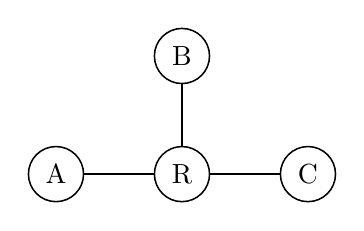
\begin{tikzpicture}[every node/.style={draw,circle,minimum size=7mm,inner sep=0pt},line width=.55pt]
\node (A) at (0,0) {A};
\node (R) at (1.6,0) {R};
\node (C) at (3.2,0) {C};
\node (B) at (1.6,1.5) {B};
\draw (A)--(R)--(C);
\draw (B)--(R);
\end{tikzpicture}
\par 图 2
\end{minipage}}
\begin{enumerate}
\item[\tikzcirclednumber{1}] R 收到来自 B 的 DV 信息：$(\mathrm{Net1},4)$、$(\mathrm{Net2},7)$、$(\mathrm{Net3},4)$，R 的路由表如何变化？
\item[\tikzcirclednumber{2}] 紧接着，R 又收到来自 A 的 DV 信息：$(\mathrm{Net2},2)$、$(\mathrm{Net3},3)$、$(\mathrm{Net5},7)$，R 的路由表如何变化？
\item[\tikzcirclednumber{3}] R 路由表根据 B 和 A 的 DV 信息更新后，使用带毒性逆转的水平分割方法向各个邻居发送自己的 DV 信息，请列出 R 发出的 DV 信息。
\end{enumerate}
\end{question}
\noindent（附录是 IPv4 的头部结构）
